\newcommand{\tableRoles}{
		\begin{center}
		\begin{tabular}{|l|c|}	 		
			\hline
			\textbf{Ruolo} &
			\textbf{Ore}\\ \hline
		}
\newcommand{\tableRolesTwo}{
		\begin{center}
		\begin{tabular}{|l|c|c|}	 
			\hline
			\textbf{Ruolo} &
			\textbf{Ore Remunerabili} &
			\textbf{Ore Totali}\\ \hline
		}
\subsection{Suddivisione delle attività}
\label{Pianificazione}
	Date le scadenze precedentemente viste e i rischi individuati si è deciso di suddividere lo sviluppo del progetto \project{}  nelle seguenti fasi:
	\begin{itemize}
\item \textbf{Fase A (FA)};
\item \textbf{Fase B (FB)};
\item \textbf{Fase C (FC)};
\item \textbf{Fase D (FD)};
\item \textbf{Fase E (FE)}.
\end{itemize}
Ogni fase è suddivisa in varie marco-attività associate a una o più risorse; a loro volta sono scomposte in attività riportate poi nel diagramma di Gantt\glossario{} solo le principali e degne di nota.
Nel Gantt\glossario{} sono riportate con colori diversi rispetto ad altre, le attività che attendono la terminazione di altre per poter partire: se dunque un'attività principale ritardasse nell'essere terminata, a sua volta porterebbe un ritardo a cascata sulle attività ad essa correlate direttamente o indirettamente.
Nel Gantt\glossario{} vengono inoltre riportate:
\begin{itemize}
\item \textbf{Milestone}\glossario: ha durata pari a zero e rappresenta, internamente, la data di conclusione delle attività previste per quella determinata fase, che si concluderà poi con la consegna dei rispettivi documenti (indicata nel Gantt\glossario{} con
il rombo rosso). Esternamente, rappresenta la revisione corrispondente alla relativa consegna o l’approvazione di quanto fatto fino a quel momento (indicata nel Gantt\glossario{} con il rombo arancione);
\item \textbf{Macro-attività:} indicate nel Gantt\glossario{} con una linea spessa orizzontale di colore nero, è un'attività che viene suddivisa al suo interno in altre piccole attività.
\end{itemize}
Si è deciso di non riportare i diagrammi PERT\glossario{} in quanto poco leggibili a causa della moltitudine di nodi presenti e in quanto non tengono conto delle risorse che si hanno a disposizione. Si è dunque pensato di fornire solamente i diagrammi Gantt\glossario{} mostrando anche l'utilizzo delle risorse a disposizione nelle varie attività.

\subsubsection{Descrizione fase A (FA)}
\label{Analisi(FA)}
Periodo: dal 2013-12-02 al 2013-12-20. \\
Questa fase inizia con la scelta del capitolato e termina con la scadenza per consegna della documentazione.
Le macro-attività di questa fase sono:
\begin{itemize}
\item \textbf{Norme di Progetto (NP):} l'\administrator{} redige le norme che i membri del gruppo \authorName{} dovranno seguire durante tutto il corso del progetto nello svolgimento delle attività a cui sono stati assegnati. Tale attività sarà la prima ad iniziare in quanto le norme che riguardano la stesura dei documenti e le adozioni software sono indipendenti dal capitolato scelto. Una volta scelto il capitolato, il documento verrà arricchito dalle norme strettamente legate al capitolato. Il rispetto delle regole imposte, verrà poi certificato dai verificatori;  
\item \textbf{Studio di Fattibilità (SF):} è un'attività cruciale in quanto bloccante per l'Analisi dei Requisiti; in questa attività vengono valutati tutti i capitolati d'appalto proposti, studiandone la complessità e, in base all'interesse dei singoli componenti in ambito tecnologico e/o di sviluppo, si decide quale capitolato si andrà a realizzare;
\item \textbf{Analisi dei Requisiti (AR):} analisi approfondita del capitolato partendo dall'analisi effettuata dallo Studio di Fattibilità. Inizia dopo la verifica dello Studio di Fattibilità e si protrae fino a prima della verifica generale;
\item \textbf{Piano di Progetto (PP):} redatto dal \projectManager{} per organizzare le attività necessarie da svolgere e assegnarle poi alle risorse in modo tale da non sovraccaricarle e impiegando al meglio il loro tempo disponibile, rispettando le milestone\glossario{} che si sono imposte in termini di tempistiche e grado di raggiungimento;
\item \textbf{Piano di Qualifica (PQ):} redatto dal \verifier{} capo in collaborazione con l'\administrator.
\item \textbf{Glossario (G):} contiene la spiegazione di alcuni termini presenti nei documenti in modo tale da dare una spiegazione univoca ed eliminare le possibili ambiguità di significato; viene scritto in modo incrementale e parallelo dai redattori dei documenti, aggiornandolo di volta in volta che si utilizza un termine che necessita di spiegazione;
\item \textbf{Lettera di Presentazione:} lettera presentata al committente che permette a \authorName{} di partecipare alla gara d'appalto per il capitolato \project . 
\end{itemize} 
I ruoli maggiormente coinvolti sono: \administrator , \analyst{} e \verifier .
\\
\paragraph{Diagramma di Gantt: Fase A }
\label{DiagrammaAnalisi}
Il seguente diagramma di Gantt\g{} illustra la pianificazione delle attività per la fase A.
\begin{figure}[!h]
	\centering
	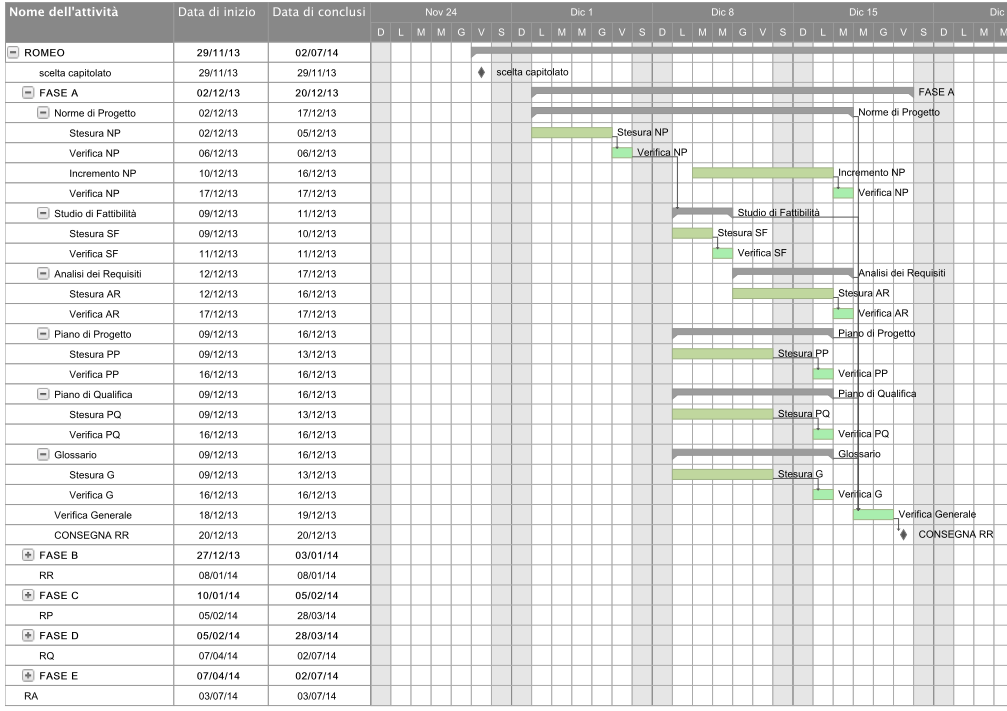
\includegraphics[width=1.2\textwidth]{./content/Immagini/faseA.png}
	\caption{Diagramma di Gantt: Fase A}
	\label{DiagrammaAnalisiGantt}
\end{figure} 
\pagebreak
\subsubsection{Descrizione fase B (FB)}
\label{Analisi Incrementale (FAI)}
Periodo: dal 2013-12-27 al 2014-01-08. \\
Questa fase inizia qualche giorno dopo la consegna e termina con la Revisione dei Requisiti (RR). In questo periodo vengono consolidati i requisiti richiesti, migliorando l’Analisi dei Requisiti e incrementando il contenuto degli altri documenti.
\paragraph{Diagramma di Gantt: Fase B }
\label{DiagrammaIncrementale}
Il seguente diagramma di Gantt\g{} illustra la pianificazione delle attività per la fase B.
\begin{figure}[h]
	\centering
	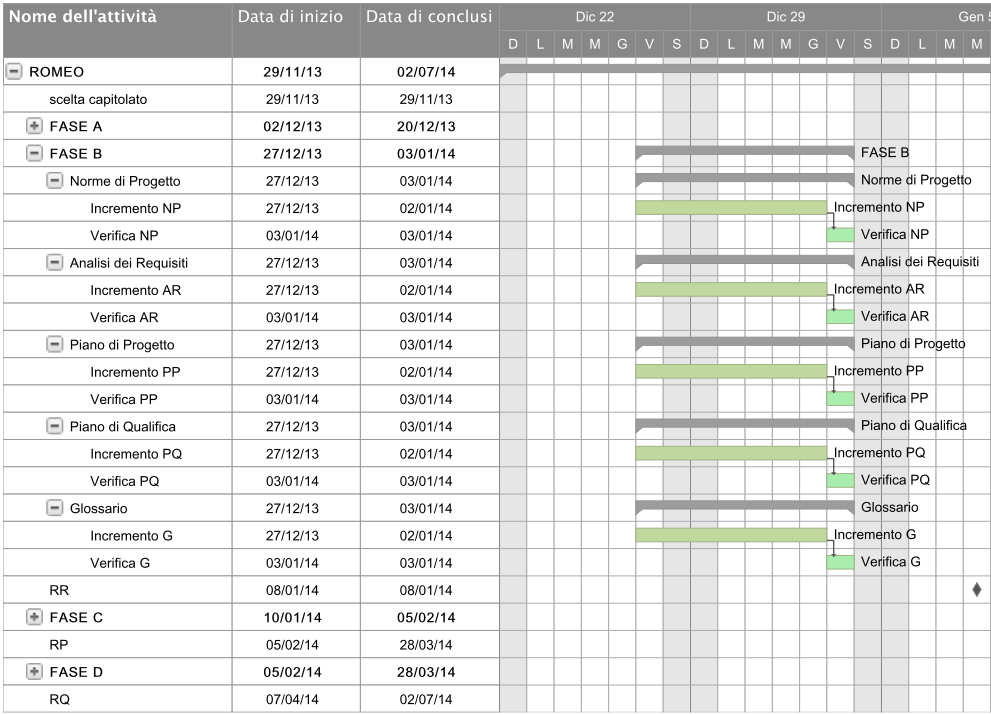
\includegraphics[width=\textwidth]{./content/Immagini/faseB.png}
	\caption{Diagramma di Gantt: Fase B}
\end{figure}
\pagebreak
\subsubsection{Descrizione fase C (FC)}
\label{Progettazione Architetturale (FPA)}
Periodo: dal 2014-01-10 al 2014-02-05. \\
Questa fase inizia con la consegna della Revisione dei Requisiti (RR) e termina con la consegna per la Revisione di Progetto (RP).
Le macro-attività di questa fase sono:
\begin{itemize}
\item \textbf{Specifica Tecnica (ST):} dove il \designer{} illustra quali sono le scelte progettuali ad alto livello che si intendono prendere in merito al prodotto che si andrà a realizzare. Verranno inoltre descritti i Design pattern\glossario{} che si utilizzeranno, l'architettura generale del software, il tracciamento dei requisiti e componenti stimandone infine risorse e costi;
\item \textbf{Incremento Documentazione:} tutti i documenti fino alla Revisione dei Requisiti realizzati verranno incrementati con il contenuto riguardante la fase C e successivamente verificati dai verificatori prima di essere consegnati per la successiva revisione (Revisione di Progettazione).
\end{itemize}
I ruoli maggiormente coinvolti sono: \designer , \verifier{} e \analyst.
\paragraph{Diagramma di Gantt: Fase C }
\label{DiagrammaArchitetturale}
Il seguente diagramma di Gantt\g{} illustra la pianificazione delle attività per la fase C.
\begin{figure}[h]
	\centering
	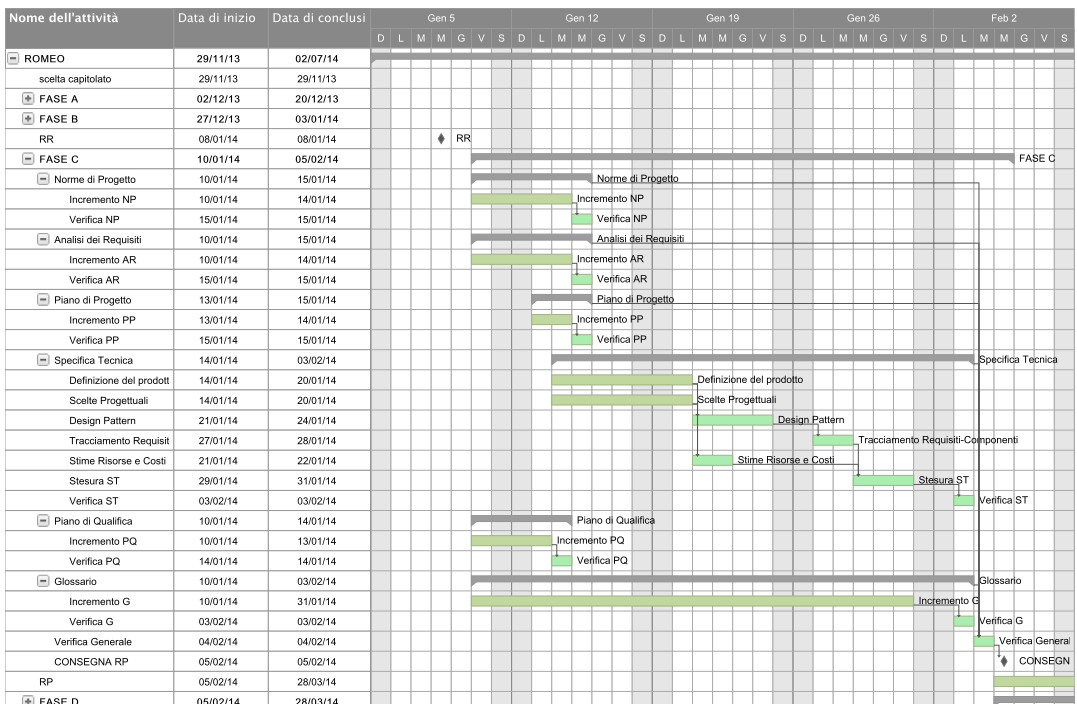
\includegraphics[width=1.2\textwidth]{./content/Immagini/faseC.png}
	\caption{Diagramma di Gantt: Fase C}
\end{figure}
\pagebreak
\subsubsection{Descrizione fase D (FD)}
\label{Progettazione di Dettaglio e Codifica (FPDC)}
Periodo: dal 2014-02-05 al 2014-03-13.\\
Questa fase inizia con la consegna della Revisione di Progetto (RP) e termina con la consegna per la Revisione di Qualifica (RQ). 
Le macro-attività di questa fase sono:
\begin{itemize}
\item \textbf{Definizione del Prodotto (DP):} in cui verranno definite in modo più approfondito la struttura e la relazione dei vari componenti che costituiscono il prodotto partendo dalla base della Specifica Tecnica (ST);
\item \textbf{Codifica (C):} questa macro-attività è stata suddivisa in due attività, in quanto, adottando un ciclo di vita incrementale, al primo ciclo, si andranno a realizzare le parti che riguardano i requisiti obbligatori mentre nel secondo quello che riguarda i requisiti opzionali che il gruppo \authorName{} vorrà soddisfare per interesse e tempo a disposizione. In questo periodo, i programmatori svilupperanno il codice del programma seguendo quanto riportato dalla Definizione del Prodotto (DP);
\item \textbf{Manuale Utente:} verrà redatto una volta finita la codifica (C) e avrà lo scopo di illustrare agli utenti coinvolti come utilizzare il sistema;
\item \textbf{Incremento Documentazione:} tutti i documenti verranno aggiornati in base all'esito della Revisione di Progetto (RP) e incrementati con il contenuto riguardante la fase D (FD).
\item \textbf{Esecuzione dei Test:} verranno eseguiti automaticamente tutti i test di unità e di integrazione previsti e codificati monitorandone i risultati.
\end{itemize}
I ruoli maggiormente coinvolti sono: \designer , \verifier{} e \programmer.
\paragraph{Diagramma di Gantt: Fase D }
\label{DiagrammaCodifica}
Il seguente diagramma di Gantt\g{} illustra la pianificazione delle attività per la fase D.
\begin{figure}[h]
	\centering
	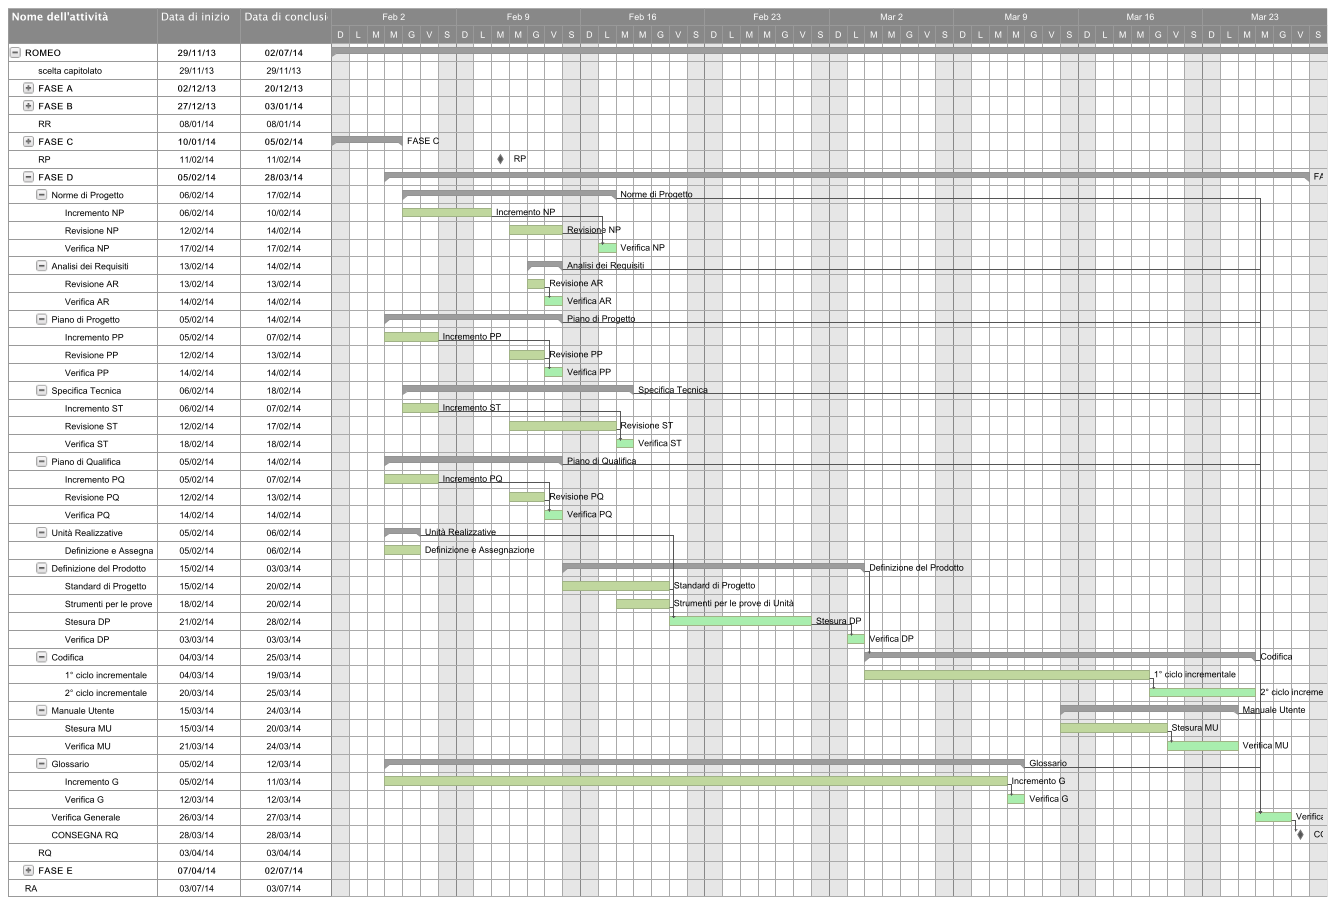
\includegraphics[width=1.2\textwidth]{./content/Immagini/faseD.png}
	\caption{Diagramma di Gantt: Fase D}
\end{figure}
\pagebreak
\subsubsection{Descrizione fase E (FE)}
\label{Verifica e Validazione (FVV)}
Periodo: dal 2014-03-13 al 2014-04-02. \\
Questa fase inizia con la consegna della Revisione di Qualifica (RQ) e termina con la consegna per la Revisione di Accettazione (RA).
Le macro-attività di questa fase sono:
\begin{itemize}
\item \textbf{Validazione Verifica e Collaudo del sistema:} in queste macro-attività, il prodotto verrà convalidato per mostrare che è conforme alle specifiche e che soddisfa i requisiti fissati e le richieste fatte dal proponente;
\item \textbf{Incremento Documentazione:} tutti i documenti verranno aggiornati in base all'esito della Revisione di Qualifica (RQ) e incrementati con il contenuto riguardante la fase E (FE).
\end{itemize}
I ruoli maggiormente coinvolti sono: \designer , \verifier{} e \programmer.
\begin{landscape}\paragraph{Diagramma di Gantt: Fase E }
\label{DiagrammaVerificaValidazione}
Il seguente diagramma di Gantt\g{} illustra la pianificazione delle attività per la fase E.
\begin{figure}[h]
	\centering
	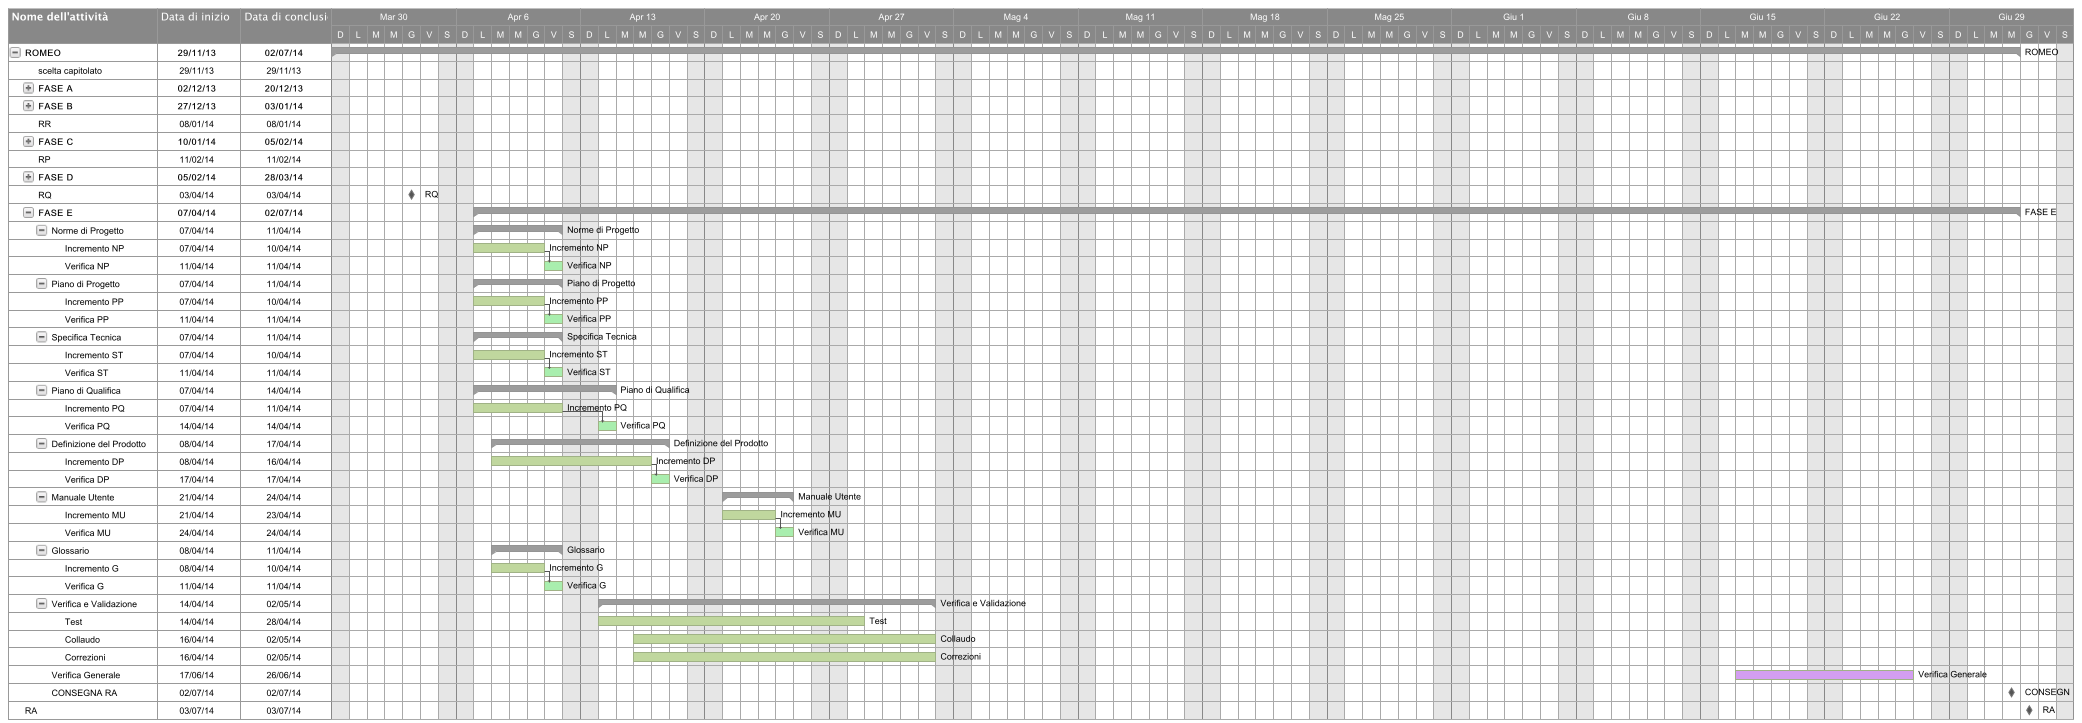
\includegraphics[width=1.2\textwidth]{./content/Immagini/faseE.png}
	\caption{Diagramma di Gantt: Fase E}
\end{figure}
\end{landscape}
\pagebreak
\subsection{Calendario attività}
\label{CalendarioAttività}
Nella sezione che segue, verranno presentati i prospetti, in forma tabulare e in forma grafica, dell'impiego dei ruoli nelle diverse fasi. Infine verranno mostrate le incidenze dei vari ruoli nel progetto nel suo complesso.
\subsubsection{Fase A}
\label{Analisi}
Le ore totali impiegate sono 144 ripartite nei seguenti ruoli:
\\
\\
\begin{table}[!h]
\tableRoles
Amministratore & 20 \\
Responsabile & 18 \\
Analista & 65 \\
Verificatore & 41 \\ \hline
\end{tabular} 
\caption{Ore a Ruolo, Fase A}
\end{center}
\end{table}
\\
\\
\\
\begin{figure}[!h]
	\centering
	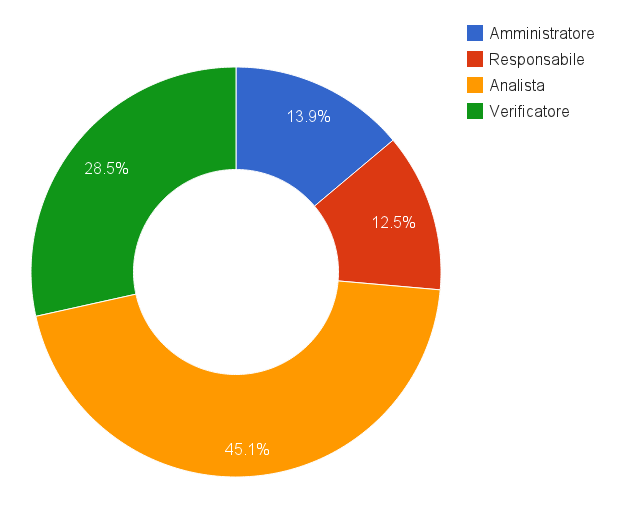
\includegraphics[width=0.9\linewidth]{./content/Immagini/prospetti/oreAn.png}
	\caption{Incidenza Ore a Ruolo, Fase A}
\end{figure}
\pagebreak
\subsubsection{Fase B}
\label{AnalisiIncrementaleR}
Le ore totali impiegate sono 59 ripartite nei seguenti ruoli:
\\
\\
\begin{table}[!h]
\tableRoles
Amministratore & 7 \\
Responsabile & 3 \\
Analista & 27 \\
Verificatore & 22 \\ \hline
\end{tabular} \caption{Ore a Ruolo, Fase B}
\end{center}
\end{table}
\\
\\
\\
\begin{figure}[h]
	\centering
	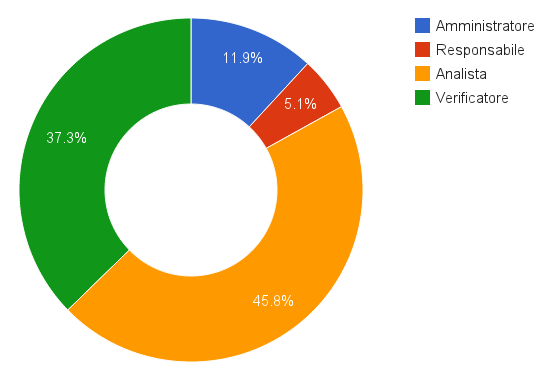
\includegraphics[width=0.9\linewidth]{./content/Immagini/prospetti/oreAnIn.png}
	\caption{Incidenza Ore a Ruolo: FB}
\end{figure} 
\pagebreak
\subsubsection{Fase C}
\label{ProgettazioneArchitetturaleR}
Le ore totali impiegate sono 183 ripartite nei seguenti ruoli:
\\
\\
\begin{table}[!h]
\tableRoles
Amministratore & 8 \\
Responsabile & 11 \\
Analista & 219 \\
Verificatore & 46 \\
Progettista & 99\\ \hline
\end{tabular} \caption{Ore a Ruolo, Fase C}
\end{center}
\end{table}
\\
\\
\\
\begin{figure}[h!]
	\centering
	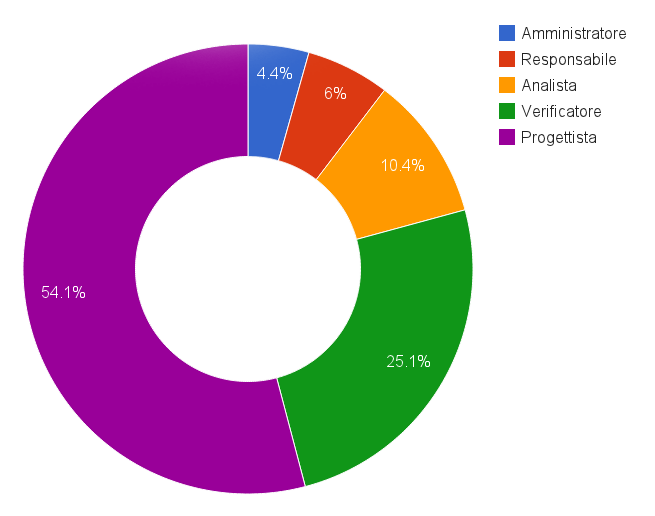
\includegraphics[width=0.9\linewidth]{./content/Immagini/prospetti/orePrAr.png}
	\caption{Incidenza Ore a Ruolo: Fase C}	
\end{figure}
\pagebreak
\subsubsection{Fase D}
\label{ProgettazioneDettaglioR}
Le ore totali impiegate sono 357 ripartite nei seguenti ruoli:
\\
\\
\begin{table}[!h]
\tableRoles
Amministratore & 9 \\
Responsabile & 11 \\
Analista & 3 \\
Verificatore & 111 \\
Progettista & 105\\
Programmatore & 118\\  \hline
\end{tabular} \caption{Ore a Ruolo, Fase D}
\end{center}
\end{table}
\\
\\
\\
\begin{figure}[h!]
	\centering
	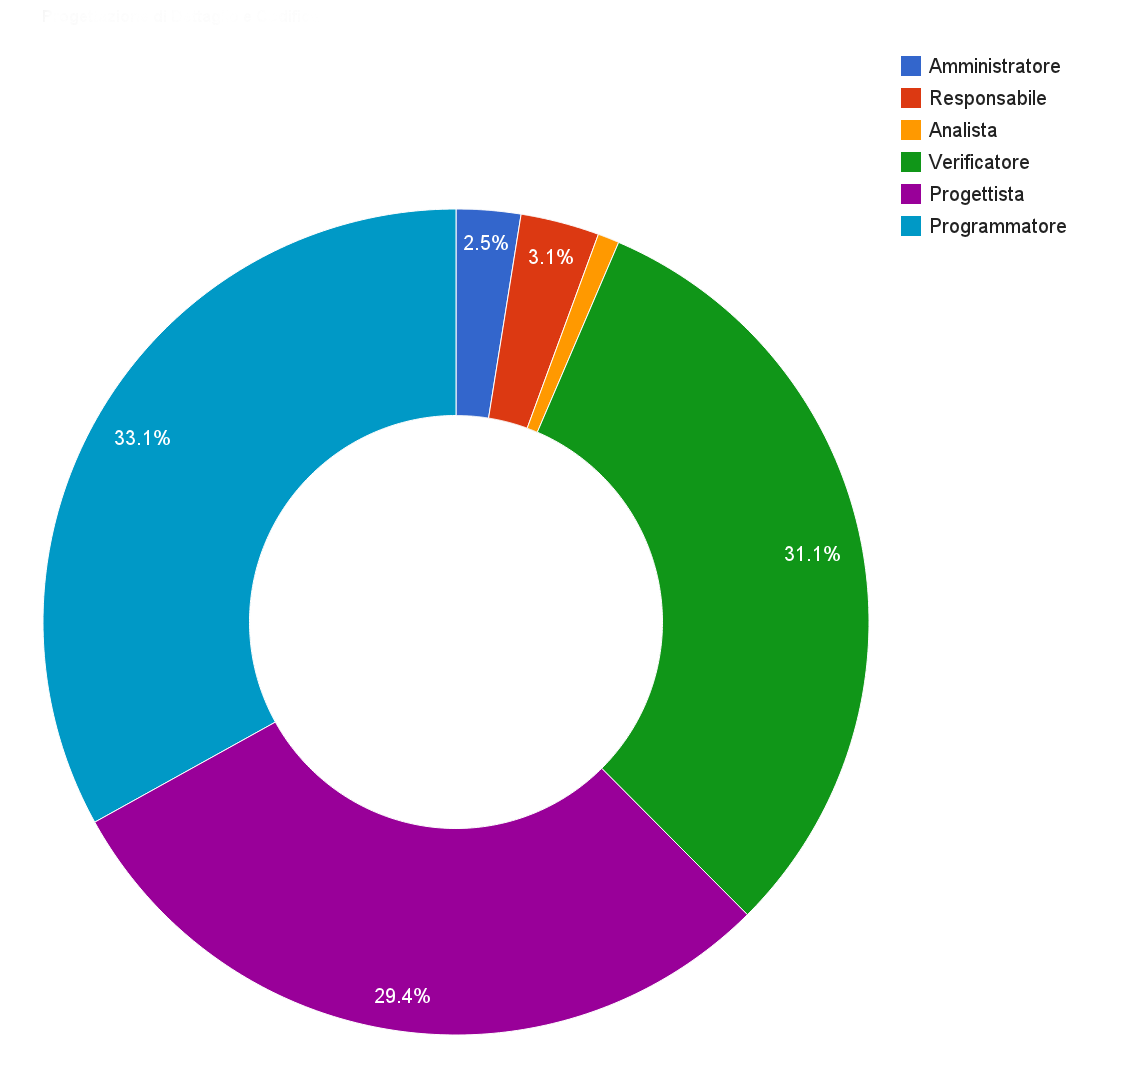
\includegraphics[width=0.9\linewidth]{./content/Immagini/prospetti/orePrDe.png}
	\caption{Incidenza Ore a Ruolo: Fase D}
\end{figure}  
\pagebreak
\subsubsection{Fase E}
\label{VerificaValidazioneR}
Le ore totali impiegate sono 111 ripartite nei seguenti ruoli:
\\
\\
\begin{table}[!h]
\tableRoles
Amministratore & 9 \\
Responsabile & 7 \\
Verificatore & 61 \\
Progettista & 20\\
Programmatore & 14\\  \hline
\end{tabular} \caption{Ore a Ruolo, Fase E} \end{center}
\end{table}
\\
\\
\\
\begin{figure}[h!]
	\centering
	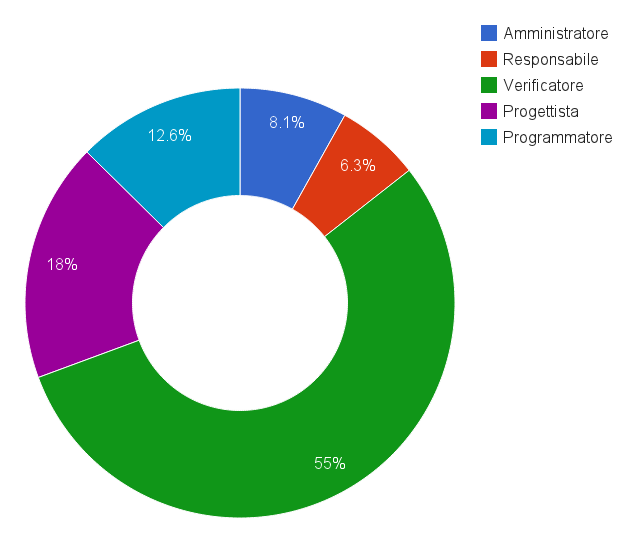
\includegraphics[width=0.9\linewidth]{./content/Immagini/prospetti/oreVV.png}
	\caption{Incidenza Ore a Ruolo: Fase E}
\end{figure}
\pagebreak
\subsubsection{Quadro riassuntivo}
\label{QuadroRiassuntivoR}
Le ore totali impiegate per lo sviluppo dell'intero progetto sono 854, di cui remunerabili 710, ripartite nei seguenti ruoli:
\begin{table}[!h]
\tableRolesTwo
Amministratore & 53 & 33 \\
Responsabile & 50 & 32\\
Analista & 114 & 49\\
Verificatore & 281 & 240\\
Progettista & 224 & 224\\
Programmatore & 132 & 132\\ \hline
\end{tabular}\caption{Ore a Ruolo, Quadro Riassuntivo}\end{center}
\end{table}
\begin{figure}[h]
	\centering
	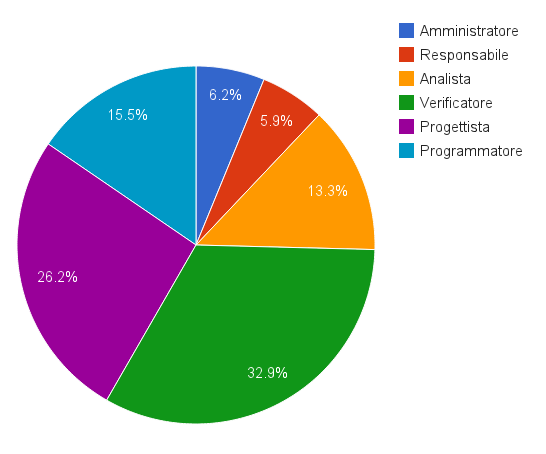
\includegraphics[width=0.48\linewidth]{./content/Immagini/prospetti/oreTotconInv.png}
	\caption{Incidenza Ore a Ruolo: Totali}
\end{figure}
\begin{figure}[h]
	\centering
	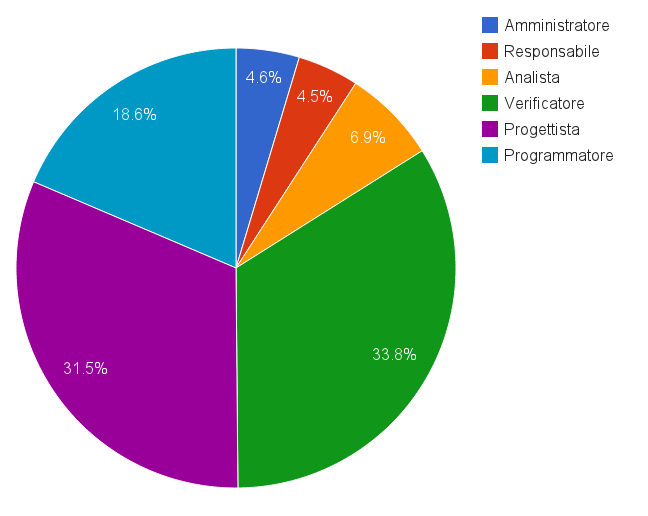
\includegraphics[width=0.48\linewidth]{./content/Immagini/prospetti/orearuoRemun.png}
	\caption{Incidenza Ore a Ruolo: Remunerabili}
\end{figure}